\begin{frame}{\subsecname: Variabili indipendenti \citep{DBLP:books/sp/Serazzi24}}
\begin{itemize}
    \item Distribuzioni di probabilità dei servizi: Esponenziali
    \item Distribuzioni di probabilità degli arrivi esterni: Esponenziali
    % TODO: \item Tempi di servizio medi per classe di job in ogni nodo
    \item Rate medi di arrivi esterni: valori che spaziano da 0.50 a 1.20 con un passo di 0.05 $job/s$, per poi estendere fino a 1.40 $job/s$ nel caso di carico pesante
    \item  Politiche di scheduling: PS
    % matrice di routing
\end{itemize}

\begin{figure}
    \centering
    \begin{subfigure}{0.49\linewidth}
        \centering
        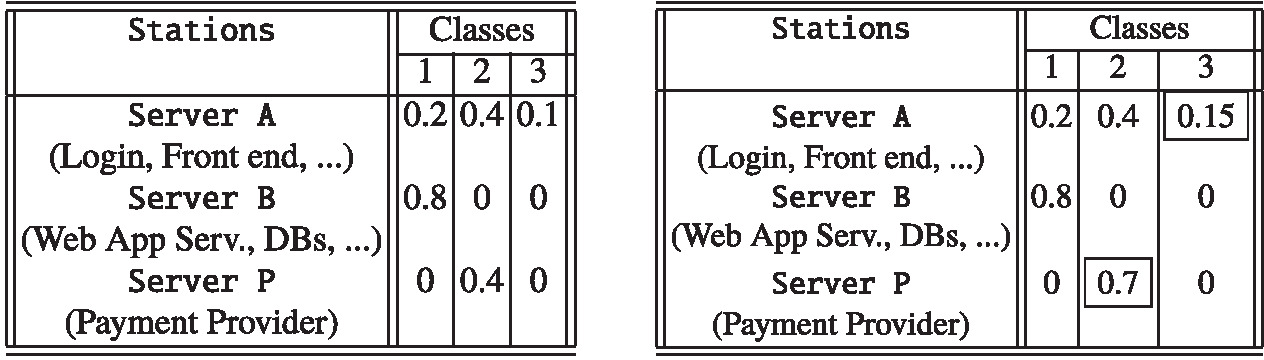
\includegraphics[width=1\linewidth]{figs/average_service_per_job_class_by_node.png}
        \caption{Tempi di servizio medi per classe di job in ogni nodo, nella versione vanilla (sinistra) e con 2FA (destra).}        
    \end{subfigure}
    \begin{subfigure}{0.49\linewidth}
        \centering
        % Please add the following required packages to your document preamble:
% \usepackage{graphicx}
% \usepackage[table,xcdraw]{xcolor}
% Beamer presentation requires \usepackage{colortbl} instead of \usepackage[table,xcdraw]{xcolor}
\begin{table}[]
\centering
\caption{Routing Matrix per jobs di una certa classe che arrivano in un server.}
\label{tab:routing-matrix}
\resizebox{\columnwidth}{!}{%
\begin{tabular}{
>{\columncolor[HTML]{FFFFFF}}l |
>{\columncolor[HTML]{FFFFFF}}l |
>{\columncolor[HTML]{FFFFFF}}l |
>{\columncolor[HTML]{FFFFFF}}l |}
\cline{2-4}
{\color[HTML]{222222} }                                                       & {\color[HTML]{222222} class 1}           & {\color[HTML]{222222} class 2}           & {\color[HTML]{222222} class3}        \\ \hline
\multicolumn{1}{|l|}{\cellcolor[HTML]{FFFFFF}{\color[HTML]{222222} Server A}} & {\color[HTML]{222222} \textbf{Server B}} & {\color[HTML]{222222} \textbf{Server P}} & {\color[HTML]{222222} \textbf{EXIT}} \\ \hline
\multicolumn{1}{|l|}{\cellcolor[HTML]{FFFFFF}{\color[HTML]{222222} Server B}} & {\color[HTML]{222222} \textbf{Server A}} & {\color[HTML]{222222} }                  & {\color[HTML]{222222} }              \\ \hline
\multicolumn{1}{|l|}{\cellcolor[HTML]{FFFFFF}{\color[HTML]{222222} Server P}} & {\color[HTML]{222222} }                  & {\color[HTML]{222222} \textbf{Server A}} & {\color[HTML]{222222} }              \\ \hline
\end{tabular}%
}
\end{table}
    \end{subfigure}
    % \caption{Caption}
    \label{fig:enter-label}
\end{figure}

\end{frame}

\begin{frame}{\subsecname: Variabili dipendenti}
    \begin{itemize}
        \item Tempo di risposta $T$: Calcolato come differenza temporale tra istante di entrata e di uscita di una richiesta in un nodo
        \item Popolazione $N$: Numero richieste all'interno di un nodo
        \item Throughput $X$: Numero di richieste soddisfatte sull'unità di tempo dal nodo
        \item Utilizzazione $\rho$: Proporzione di tempo in cui il nodo è occupato a smaltire richieste durante un periodo di osservazione
    \end{itemize}
\end{frame}